\documentclass[]{article}
\usepackage{lmodern}
\usepackage{amssymb,amsmath}
\usepackage{ifxetex,ifluatex}
\usepackage{fixltx2e} % provides \textsubscript
\ifnum 0\ifxetex 1\fi\ifluatex 1\fi=0 % if pdftex
  \usepackage[T1]{fontenc}
  \usepackage[utf8]{inputenc}
\else % if luatex or xelatex
  \ifxetex
    \usepackage{mathspec}
  \else
    \usepackage{fontspec}
  \fi
  \defaultfontfeatures{Ligatures=TeX,Scale=MatchLowercase}
\fi
% use upquote if available, for straight quotes in verbatim environments
\IfFileExists{upquote.sty}{\usepackage{upquote}}{}
% use microtype if available
\IfFileExists{microtype.sty}{%
\usepackage{microtype}
\UseMicrotypeSet[protrusion]{basicmath} % disable protrusion for tt fonts
}{}
\usepackage[margin=2cm]{geometry}
\usepackage{hyperref}
\hypersetup{unicode=true,
            pdftitle={SATIATED},
            pdfauthor={Richard Pilbery},
            pdfborder={0 0 0},
            breaklinks=true}
\urlstyle{same}  % don't use monospace font for urls
\usepackage{natbib}
\bibliographystyle{apalike}
\usepackage{longtable,booktabs}
\usepackage{graphicx,grffile}
\makeatletter
\def\maxwidth{\ifdim\Gin@nat@width>\linewidth\linewidth\else\Gin@nat@width\fi}
\def\maxheight{\ifdim\Gin@nat@height>\textheight\textheight\else\Gin@nat@height\fi}
\makeatother
% Scale images if necessary, so that they will not overflow the page
% margins by default, and it is still possible to overwrite the defaults
% using explicit options in \includegraphics[width, height, ...]{}
\setkeys{Gin}{width=\maxwidth,height=\maxheight,keepaspectratio}
\IfFileExists{parskip.sty}{%
\usepackage{parskip}
}{% else
\setlength{\parindent}{0pt}
\setlength{\parskip}{6pt plus 2pt minus 1pt}
}
\setlength{\emergencystretch}{3em}  % prevent overfull lines
\providecommand{\tightlist}{%
  \setlength{\itemsep}{0pt}\setlength{\parskip}{0pt}}
\setcounter{secnumdepth}{5}
% Redefines (sub)paragraphs to behave more like sections
\ifx\paragraph\undefined\else
\let\oldparagraph\paragraph
\renewcommand{\paragraph}[1]{\oldparagraph{#1}\mbox{}}
\fi
\ifx\subparagraph\undefined\else
\let\oldsubparagraph\subparagraph
\renewcommand{\subparagraph}[1]{\oldsubparagraph{#1}\mbox{}}
\fi

%%% Use protect on footnotes to avoid problems with footnotes in titles
\let\rmarkdownfootnote\footnote%
\def\footnote{\protect\rmarkdownfootnote}

%%% Change title format to be more compact
\usepackage{titling}

% Create subtitle command for use in maketitle
\newcommand{\subtitle}[1]{
  \posttitle{
    \begin{center}\large#1\end{center}
    }
}

\setlength{\droptitle}{-2em}
  \title{SATIATED}
  \pretitle{\vspace{\droptitle}\centering\huge}
  \posttitle{\par}
  \author{Richard Pilbery}
  \preauthor{\centering\large\emph}
  \postauthor{\par}
  \predate{\centering\large\emph}
  \postdate{\par}
  \date{2019-02-21}

\usepackage{booktabs}
\usepackage{amsthm}
\makeatletter
\def\thm@space@setup{%
  \thm@preskip=8pt plus 2pt minus 4pt
  \thm@postskip=\thm@preskip
}
\makeatother
\usepackage{booktabs}
\usepackage{longtable}
\usepackage{array}
\usepackage{multirow}
\usepackage[table]{xcolor}
\usepackage{wrapfig}
\usepackage{float}
\usepackage{colortbl}
\usepackage{pdflscape}
\usepackage{tabu}
\usepackage{threeparttable}
\usepackage[normalem]{ulem}

\AtBeginDocument{\let\maketitle\relax}

\begin{document}
\maketitle

\hypertarget{soiled-airway-tracheal-intubation-and-the-effectiveness-of-decontamination-by-paramedics-satiated-a-randomised-controlled-manikin-study-}{%
\section{Soiled Airway Tracheal Intubation and the Effectiveness of
Decontamination by Paramedics (SATIATED): A randomised controlled
manikin
study-}\label{soiled-airway-tracheal-intubation-and-the-effectiveness-of-decontamination-by-paramedics-satiated-a-randomised-controlled-manikin-study-}}

\hypertarget{author-information}{%
\subsection{Author information}\label{author-information}}

\textbf{Richard Pilbery}\\
Research paramedic\\
Yorkshire Ambulance Service NHS Trust\\
Springhill, Brindley Way\\
Wakefield 41 Business Park\\
Wakefield\\
WF2 0XQ

ORCID: \url{https://orcid.org/0000-0002-5797-9788}

email: \href{mailto:r.pilbery@nhs.net}{\nolinkurl{r.pilbery@nhs.net}}\\
tel:

\textbf{Dr.~M. Dawn Teare}\\
Reader in Epidemiology and Biostatistics\\
University of Sheffield

\textbf{Word count:} 2707

\textbf{Keywords:} Keyword 1, keyword 2, keyword 3

\hypertarget{abstract}{%
\subsection{Abstract}\label{abstract}}

\hypertarget{introduction}{%
\subsubsection{Introduction}\label{introduction}}

Intro

\hypertarget{methods}{%
\subsubsection{Methods}\label{methods}}

Methods

\hypertarget{results}{%
\subsubsection{Results}\label{results}}

Results

\hypertarget{conclusion}{%
\subsubsection{Conclusion}\label{conclusion}}

Conclusion

\hypertarget{intro}{%
\section{Introduction}\label{intro}}

Vomiting and regurgitation are commonly encountered in
out-hospital-cardiac arrest with a reported incidence of 20--30\%
\citep{voss_how_2014, simons_incidence_2007}. This is of concern since
patients who have suffered an OHCA, are already in extremis. If standard
suctioning techniques are not sufficient to maintain a clear airway and
provide ventilation, then these patients will die, irrespective of the
quality of chest compressions and the timeliness of defibrillation.
Arguably, tracheal intubation is the preferred airway management
technique in patients with ongoing airway contamination, but there is
evidence that this is difficult to achieve when the airway is soiled
\citep{sakles_impact_2017}. Even if patients survive to the hospital, it
is possible that aspiration pneumonias may adversely affect survival
outcome, although this has yet to be proved empirically
\citep{christ_early-onset_2016}.

Traditional suctioning techniques have been criticised, and training in
the management of contaminated airways, limited. This has led to the
development of a combined suction/laryngoscopy technique to facilitate
intubation, known as Suction Assisted Laryngoscopy and Airway
Decontamination (SALAD), and the creation of modified airway manikins to
allow for practice in these techniques \citep{ducanto_novel_2017}.

However, to date there has only been one study specifically looking at
the SALAD technique and the outcomes limited to self-reported confidence
measures of trainees in using the technique. Other techniques have been
described to manage significant airway contamination, including the use
of a meconium aspirator \citep{kei_comparing_2017}, although this
technique is not practical in the out-of-hospital environment (and
requires a device that is not typically carried by UK ambulance
services), and deliberate intubation of the oesophagus (the oesophageal
diversion manoeuvre), of which the sum total of evidence in support of
the procedure is a single case report \citep{kornhall_intentional_2015}.

This study aims to determine whether a short teaching session of the
SALAD technique to paramedics, improves their ability to intubate a
contaminated airway.The primary objective is to determine the difference
between paramedic first-pass intubation success, before and after SALAD
training, in a simulated soiled airway. Secondary objectives are to
determine the difference in time taken to achieve first-pass intubation
success, before and after SALAD training in a simulated soiled airway,
and the effect of multiple intubation attempts on success rates
following SALAD training.

\hypertarget{methods-1}{%
\section{Methods}\label{methods-1}}

\hypertarget{study-design-and-participants}{%
\subsection{Study design and
participants}\label{study-design-and-participants}}

This randomised controlled trial was conducted in Yorkshire Ambulance
Service NHS Trust (YAS). Participants were NHS staff employed by YAS,
who were Health and Care Professions Council (HCPC) registered
paramedics at the time of enrolment in the study, authorised to intubate
and who had received no SALAD training in the previous 3 months.
Potential participants were excluded if they did not meet the inclusion
criteria, were allergic to the `vomit' ingredients or unwilling to
provide consent to participate.

\hypertarget{randomisation}{%
\subsection{Randomisation}\label{randomisation}}

In order to adjust for changes in participant performance that might
arise from repeated attempts at intubation, paramedics were randomised
into either: making two pre-training intubation attempts and one
post-training attempt (group AAB); or making one pre-training intubation
attempt and two post-training attempts (ABB). Groups were evenly
allocated (i.e.~1:1) using a block randomisation sequence provided by
RANDOM.ORG. To distinguish between the training pathways and number of
the assessed attempts, group AAB's attempts were denoted
A\textsubscript{01}A\textsubscript{02}B\textsubscript{01} and group
ABBs, A\textsubscript{11}B\textsubscript{11}B\textsubscript{12}. It was
not possible to blind participants or the researcher from the group
allocation.

\hypertarget{intervention}{%
\subsection{Intervention}\label{intervention}}

\hypertarget{salad-manikin}{%
\subsubsection{SALAD manikin}\label{salad-manikin}}

A modified TruCorp AirSim Advance airway manikin was used for the study
as it has realistic airway anatomy and can be used for tracheal
intubation training. The oesophagus of this manikin has been connected,
via a hosepipe, to a bilge pump that is sited within a reservoir of
simulated vomit (Figure \ref{fig:figure1}). The vomit is water, coloured
with food-grade colouring, and thickened with xanthan gum (a food
additive). Once the bilge pump is switched on, it can generate a
constant flow of liquid into the oropharynx, obscuring any view of the
laryngeal inlet. The flow rate is controlled by a tap, which was
calibrated to provide 1 L/min of vomit to the oropharynx of the manikin
during intubation attempts. To keep vomit within the oropharynx, the
left and right bronchi on the manikin have been occluded.

Standard intubation equipment, including personal protective equipment
(PPE) and motorised suction, that is routinely used within YAS was
provided for participants, and the study researcher acted as a competent
assistant for the intubation attempts.

\begin{figure}
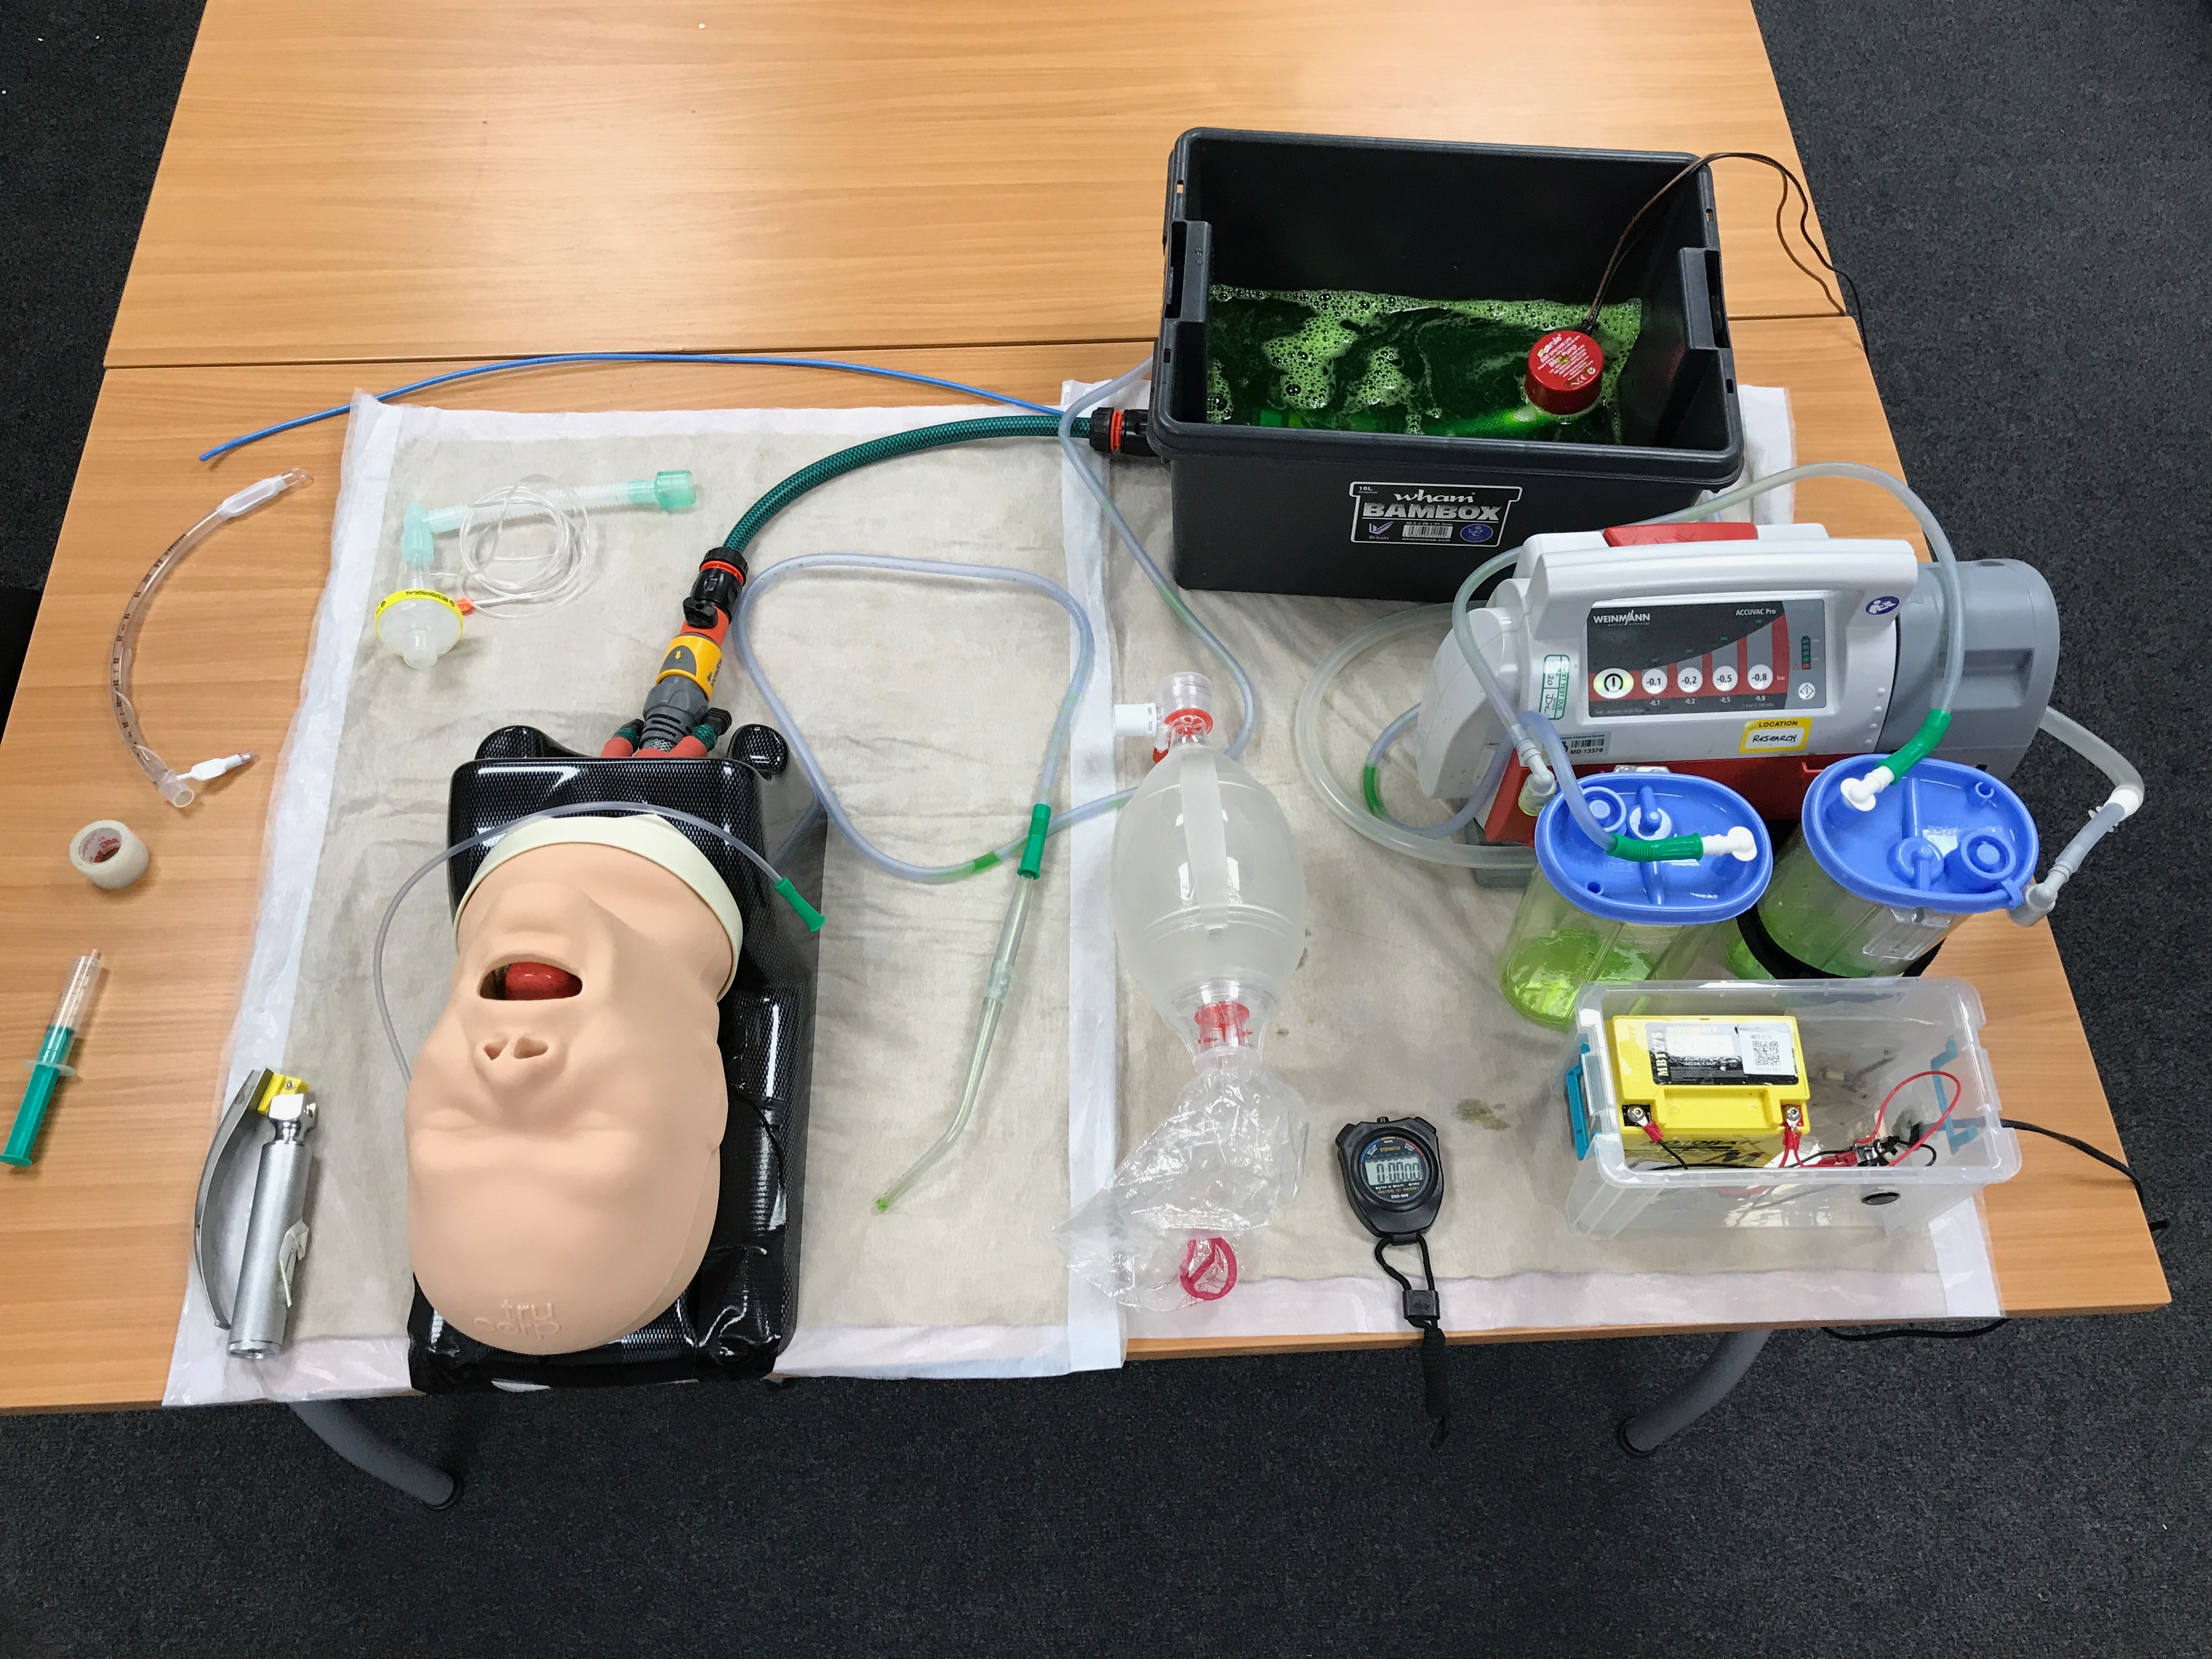
\includegraphics[width=7in]{images/figure-1} \caption{SALAD manikin setup used for the study}\label{fig:figure1}
\end{figure}

\hypertarget{procedure}{%
\subsubsection{Procedure}\label{procedure}}

Once informed consent was obtained, paramedics were randomised into
either group AAB or ABB. All attempts utilised direct laryngoscopy,
which is the standard intubation technique within YAS. Prior to each
intubation attempt, the manikin was primed with vomit to ensure the same
level of oropharyngeal obstruction. All attempts were video recorded for
timing accuracy.

Participants were deemed to have begun their attempt once the bilge pump
was turned on. The attempt was considered to be over when either: the
paramedic intubated the manikin and verbally confirmed with the
researcher that the attempt had been completed or; 90 seconds had
elapsed or; the tracheal tube was placed into the oesophagus and the
cuff inflated while the pump was still running.

If the tracheal tube was not in the trachea, with the cuff inflated and
connected to a bag-valve device within 90 seconds, the attempt was
considered a failure.

Participants randomised into the two pre-training attempts group (AAB)
made their second intubation attempt immediately following the first,
and prior to the group training session. Once all participants completed
their pre-training intubation attempt(s), the training session was
delivered. The training intervention adopted the Advanced Life Support
Group/Resuscitation Council 4-stage approach of skills teaching,
comprising \citep{bullock_pocket_2008}:

\begin{enumerate}
\def\labelenumi{\arabic{enumi}.}
\tightlist
\item
  A real-time demonstration of the SALAD technique by the researcher
\item
  A repeated demonstration with an explanation of the rationale of the
  steps taken when performing SALAD (not real-time)
\item
  Another demonstration of the SALAD technique conducted by the
  researcher, but guided by one of the participants
\item
  An attempt by the same participant who guided the researcher in the
  previous step, followed by a practice attempt by the other
  participants.
\end{enumerate}

Following the training session, participants made their post-training
intubation attempt(s) conducted using the same method as for the
pre-training intubation attempt(s). Participants randomised into the two
post-training attempts (ABB), made their second attempt immediately
following the first post-training attempt.

\hypertarget{outcomes}{%
\subsection{Outcomes}\label{outcomes}}

The primary outcome was the difference in proportions of paramedic
first-pass intubation success, before and after SALAD training.

The secondary outcomes were:

\begin{itemize}
\tightlist
\item
  Mean of the differences between groups AAB and ABB with respect to the
  first and second successful intubation attempt times, and between the
  first and third successful intubation attempt times
\item
  Difference in success rates between participants who have two
  post-training intubation attempts (ABB) versus participants who only
  have one post-training intubation attempt (AAB).
\end{itemize}

\hypertarget{statistical-analysis}{%
\subsection{Statistical analysis}\label{statistical-analysis}}

\hypertarget{sample-size}{%
\subsection{Sample size}\label{sample-size}}

A sample size of 154 participants was calculated to be required to
detect a change in the proportion of intubation successes, from 0.25 in
the pre-training group, to 0.50 in post-training group, with a power
(1-\(\beta\)) of 90\% and a significance level (\(\alpha\)) of 5\%.
Given that there is no literature to guide expected performance, a
conservative estimate was made in consultation with an internationally
recognised SALAD expert, Dr.~James DuCanto (J.DuCanto, personal
communication, April 26, 2018).

\hypertarget{primary-outcome-analysis}{%
\subsubsection{Primary outcome
analysis}\label{primary-outcome-analysis}}

To determine if the training had an effect and increased the success
rate of intubation, the proportions of success in the groups who
received no training before their 2nd intubation attempt
(A\textsubscript{02}) was compared to those who did receive training
before their 2nd intubation attempt (B\textsubscript{11}). Comparing the
rates at these time points, controlled for any learning effect due to
participants making more than one attempt at intubation. The difference
in the two proportions was analysed using a two independent samples
proportion z-test, assuming a two-sided type 1 error rate of 5\%.

\hypertarget{secondary-outcome-analysis}{%
\subsubsection{Secondary outcome
analysis}\label{secondary-outcome-analysis}}

Only successful intubation attempts and their timings were included in
the secondary outcome analysis. The mean of the attempt time differences
(A\textsubscript{01} -- A\textsubscript{02}) were compared with the mean
of attempt time differences (A\textsubscript{11} --
B\textsubscript{11}). In addition, the mean of the attempt time
differences seen at the final measurements, (A\textsubscript{01} --
B\textsubscript{01}) were compared to (A\textsubscript{11} --
B\textsubscript{12}), to see if there were any differences between the
two pathways, which might suggest that practice following the training,
further improved the time to successful intubation. In addition, success
rates between B\textsubscript{01} and B\textsubscript{12} attempts were
compared to see whether practice following training improved the
intubation success rate. A Student's t-test was utilised to test for the
differences between mean pre- and post-training intubation attempt
times, and a two independent samples proportion z-test to test the
difference in success rates.

\hypertarget{results-1}{%
\section{Results}\label{results-1}}

164 participants took part in SATIATED, with an equal number in groups
AAB and ABB. The groups were similar with respect to intubation attempts
(successful or not) undertaken in the previous 12 months. The median
number of years as a paramedic was 1.5 years less in group ABB, although
the interquartile range was similar. 36 participants had heard of the
SALAD technique prior to the study, with a slightly higher number in
group ABB (Table \ref{tab:demoTable}).

\rowcolors{2}{gray!6}{white}
\begin{table}

\caption{\label{tab:demoTable}Summary details of participants}
\centering
\begin{tabular}[t]{llll}
\hiderowcolors
\toprule
Measure & AAB & ABB & Total\\
\midrule
\showrowcolors
n & 82 & 82 & 164\\
Median intubation attempts in past 12 months (IQR) & 2.5 (0-6) & 3.0 (1-7) & 3.0 (1-6.5)\\
Median number of successful intubation attempts in past 12 months (IQR) & 2 (0-5) & 2 (0-6) & 2 (0-6)\\
Median years as paramedic (IQR) & 5.0 (1-10) & 3.5 (0-10) & 4.0 (1-10)\\
Familiar with SALAD technique & 15 & 21 & 36\\
\bottomrule
\end{tabular}
\end{table}
\rowcolors{2}{white}{white}

First-pass intubation success with and without SALAD on the second
attempt, was 53.7\% vs 90.2\% respectively, a significant difference of
36.6\% (95\%CI 24--49.1\%, p\textless{}0.0001).

Figure \ref{fig:boxplotint} summarises the intubation attempt times by
participants in each randomisation group. For successful intubation
attempts, group ABB was generally faster, except on attempt 2, where AAB
intubated sooner (Table \ref{tab:summarytime}.

\rowcolors{2}{gray!6}{white}
\begin{table}

\caption{\label{tab:summarytime}Summary data of the differences between successful intubation attempts}
\centering
\begin{tabular}[t]{>{\raggedright\arraybackslash}p{4cm}llllll}
\hiderowcolors
\toprule
\multicolumn{1}{c}{ } & \multicolumn{2}{c}{Attempt 1} & \multicolumn{2}{c}{Attempt 2} & \multicolumn{2}{c}{Attempt 3} \\
\cmidrule(l{2pt}r{2pt}){2-3} \cmidrule(l{2pt}r{2pt}){4-5} \cmidrule(l{2pt}r{2pt}){6-7}
Measure & AAB & ABB & AAB & ABB & AAB & ABB\\
\midrule
\showrowcolors
Successful attempts n (\%) & 29 (35.4) & 31 (37.8) & 44 (53.7) & 74 (90.2) & 71 (86.6) & 73 (89)\\
Median elapsed time to intubation attempt secs (IQR) & 7 (4--13) & 6 (3--11) & 4 (2--8.5) & 4 (2--6) & 4 (2--5.5) & 3 (2--5)\\
Median intubation attempt time secs (IQR) & 54 (46--61) & 50 (40.5--58.5) & 40.5 (32.5--57.5) & 44 (39--53) & 47 (40--54) & 41 (35--50)\\
Median total attempt time secs (IQR) & 63 (52--74) & 59 (48.5--70.5) & 49 (37.5--61.5) & 47.5 (43--58) & 51 (43.5--58) & 44 (38--52)\\
\bottomrule
\multicolumn{7}{l}{\textbf{Note: } }\\
\multicolumn{7}{l}{In order to be included in this table, both attempts had to be successful.}\\
\end{tabular}
\end{table}
\rowcolors{2}{white}{white}

\begin{figure}
\centering
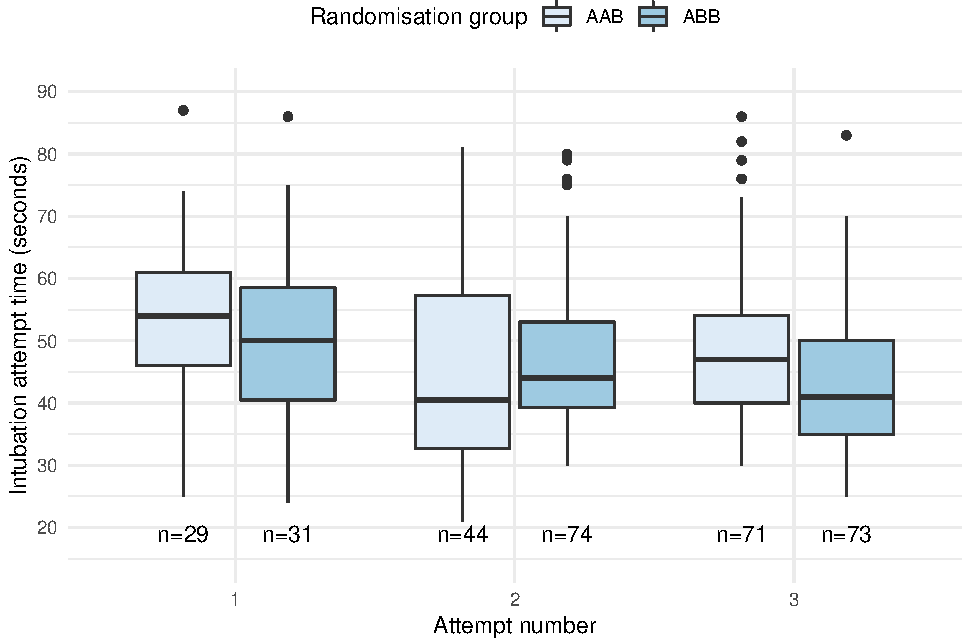
\includegraphics{SATIATED_files/figure-latex/boxplotint-1.pdf}
\caption{\label{fig:boxplotint}Intubation attempt times, stratified by
randomisation sequence and attempt}
\end{figure}

\hypertarget{mean-difference-in-successful-intubation-attempts}{%
\subsection{Mean difference in successful intubation
attempts}\label{mean-difference-in-successful-intubation-attempts}}

\rowcolors{2}{gray!6}{white}
\begin{table}

\caption{\label{tab:lotsmeans}Summary data of successful intubation attempts}
\centering
\begin{tabular}[t]{lrrrrl}
\hiderowcolors
\toprule
group & n & mean difference (secs) & standard deviation (secs) & standard error (secs) & 95\% CI\\
\midrule
\showrowcolors
\addlinespace[0.3em]
\multicolumn{6}{l}{\textbf{Attempts 1 and 2}}\\
\hspace{1em}AAB & 23 & 15.4 & 16.7 & 3.5 & 8.2--22.6\\
\hspace{1em}ABB & 28 & 3.7 & 17.9 & 3.4 & -3.3--10.6\\
\addlinespace[0.3em]
\multicolumn{6}{l}{\textbf{Attempts 1 and 3}}\\
\hspace{1em}AAB & 27 & 6.0 & 20.4 & 3.9 & -2.1--14.1\\
\hspace{1em}ABB & 27 & 8.5 & 11.5 & 2.2 & 4--13.1\\
\bottomrule
\end{tabular}
\end{table}
\rowcolors{2}{white}{white}

There was a significant difference between groups AAB (n=23) and ABB
(n=28) with respect to the mean difference in time taken to perform a
successful intubation on attempts 1 and 2 (mean difference 11.71
seconds, 95\% CI 1.95--21.47 seconds, p=0.02). There was no significant
difference between groups AAB (n=27) and ABB (n=27) with respect to mean
difference in time taken to perform a successful intubation on attempts
1 and 3 (mean difference -2.52 seconds, 95\% CI -11.64--6.61 seconds,
p=0.58)). Summary values for the mean differences are shown in Table
\ref{tab:lotsmeans}. Finally, there was no significant difference in
success rates on the third attempt between AAB and ABB 89\% vs 86.6\%
respectively, a difference of 2.4\% (95\%CI 7.6--12.4\%, p=0.63).

\hypertarget{technique}{%
\subsection{Technique}\label{technique}}

A number of techniques were utilised by participants to facillitate
intubation (Figure \ref{fig:techniqueBarchart}). This included asking
the assistant to hold the suction catheter in the mouth (n=35), and
leaving with the suction in the mouth (although without occluding the
suction vent hole, n=20). In addition, there were also instances where
participants did not use a bougie (n=48, of which 21 were successful
attempts, and 27 unsucessful) and forgot to occlude the suction vent
hole on the catheter when attempting to clear the airway themselves
(n=35).

\begin{figure}
\centering
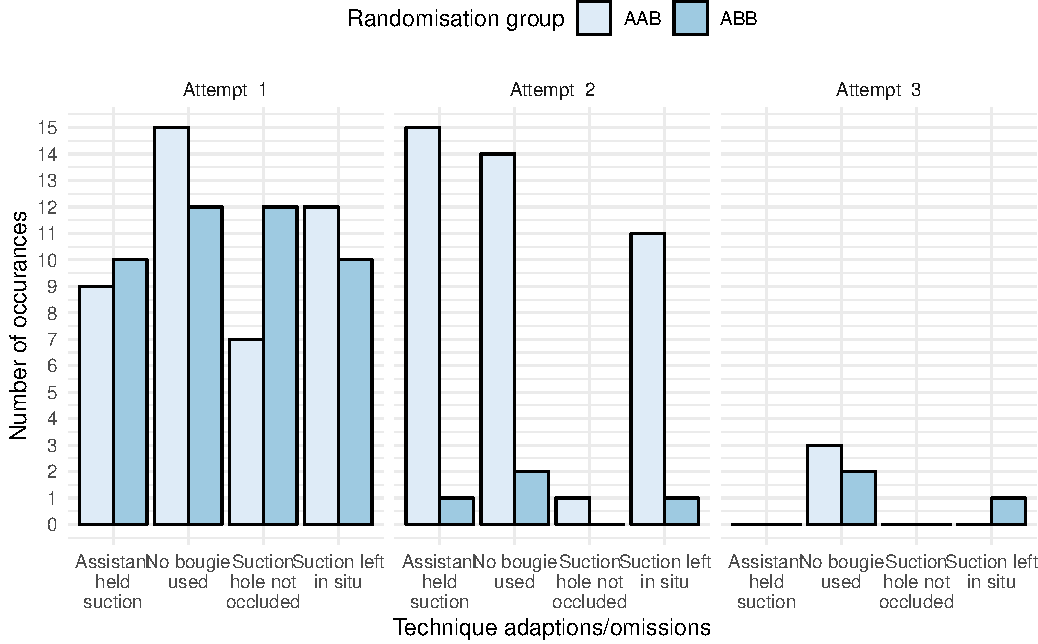
\includegraphics{SATIATED_files/figure-latex/techniqueBarchart-1.pdf}
\caption{\label{fig:techniqueBarchart}Bar chart showing techniques and
omissions during intubation attempts, stratified by randomisation group
and attempt number}
\end{figure}

\hypertarget{discussion}{%
\section{Discussion}\label{discussion}}

In this manikin study, following a brief training session, paramedics
were able to intubate a soiled airway on their first attempt,
significantly more often when using the SALAD technique (90.2\% vs
53.7\%, difference of 36.6\%, 95\%CI 24--49.1\%, p\textless{}0.001). In
addition, the mean difference in time taken to perform a successful
intubation between groups was signficant for on attempts 1 and 2 (mean
difference 11.71 seconds, 95\% CI 1.95-- 21.47 seconds, p=0.02), but not
attempts 1 and 3 (mean difference -2.52 seconds, 95\% CI -11.64--6.61
seconds, p=0.58)). There was no significant difference in success rates
on the third attempt between AAB and ABB (89.0\% vs 86.6\%, difference
2.4\%, 95\%CI 7.6--12.4\%, p=0.63).

\hypertarget{salad}{%
\subsection{SALAD}\label{salad}}

While evolution of the SALAD technqiue has occured as knowledge of the
technique has spread, the essential principles as described by Jim
DuCanto remain the same {[}REF{]}:

\begin{enumerate}
\def\labelenumi{\arabic{enumi}.}
\tightlist
\item
  Correct positioning of the patient for intubation success
  (e.g.~external auditory meatus level with sternal notch)
\item
  Holding the suction catheter (wide-bore, rigid) in a clenched-fisted
  right hand, with the distal end of the catheter pointing caudad and
  posterior, to enable manipulation of the tongue and mandible as
  required
\item
  Leading with suction to enable identifcation of relevant anatomical
  structure (posterior portion of tongue, epiglottis, vallecular and
  laryngeal outlet) and following with the laryngoscope (particularly
  important with video laryngoscopes to avoid contaminating the optics)
\item
  Once the laryngoscope is in the vallecular and a view of the laryngeal
  inlet has been obtained, the suction catheter is `parked' in the top
  of the oesophagus to provide continuous suction during the remainder
  of the intubation attempt
\item
  In order to facillitate placement of the tracheal tube, the suction
  catheter is moved across to the left-side of the mouth, which
  remaining in the oesophagus. This can be achieved by either sliding
  the catheter under the laryngoscope blade, or by briefly removing the
  catheter and inserting it to the left of the laryngoscope blade
\item
  Intubate as normal, with or without a bougie
\item
  Inflate the cuff on the tracheal tube to prevent further contamination
  of the lower airway
\item
  Suction down the tracheal tube with a flexible suction catheter prior
  to ventilation.
\end{enumerate}

The last step in this process typically takes 7--10 seconds to complete,
a fact that was overlooked during the design of this study as has likely
confounded the mean timing differences aimed at identification learning
that occured from multiple attempts. None of the pre-training attempts
finished with post-intubation suction, whereas 100\% of the
post-training attempts did. Successful intubations in group AAB did show
timinig improvements between attempts 1 and 2, but the delay in
intubation completion in the latter attempts, might explain why there
appears to be no significant difference between attempts 1 and 3.

\hypertarget{suction-catheters}{%
\subsection{Suction catheters}\label{suction-catheters}}

The suction catheters used by YAS (Penine healthcare Link Yankauer 22ch
with 6mm internal diameter tubing) have an internal diameter of
approximately 6mm and include a vent hole. For this study, the vent hole
was occluded by tape for the training and post-training attempts.
Failure to occlude the vent hole did occur on occasion during some
attempts, and this has been reported elsewhere.
\citet{cox_yankauer_2017} conducted a simulated soiled airway study with
37 emergency medicine residents, and found that 76\% did not occlude the
vent hole immediately on suctioning, with 60\% having to be prompted to
do so after 20 seconds. Catheters are available which do not contain a
vent hole, which may make them more suitable for emergency situations.

Occluding the vent hole also presented a challenge for participants who
left the suction in situ while continiuing with an intubation attempt.
While this strategy did make it easier to recommence suction when the
vent hole was re-occluded by the participant, for the remainder of the
attempt, the suction catheter restricted the view of the oropharynx. One
alternative strategy that some participants did use, was to utilise the
assistant to hold the suction in the oropharynx, thus maintaining
continuous suction.

\hypertarget{bougies}{%
\subsection{Bougies}\label{bougies}}

The Trust mandates the use of bougies as part of the intubation standard
operating procedure. Bougies have been associated with improved
first-pass intubation success
\citep{kingma_comparison_2017, driver_bougie_2017} in other studies. In
YAS, paramedics are generally taught to `railroad' the tracheal tube
following successful bougie insertion through the vocal cords. Stylets
are not used. In this study, most attempts did use a bougie, with the
exception of

\hypertarget{limitations}{%
\subsection{Limitations}\label{limitations}}

This was a manikin study and as such, does not reflect clinical
practice. For paramedics, most intubations they attempt will be at floor
level and occur during a cardiac arrest, which is likely to result in
some head and neck movement. The intubation attempts in the study by
contrast were conducted on a static manikin at table height. In
addition, the manikin could not be moved, so alternatrive positioning
such as lateral head movement, or placing the patient in a Tredelenburg
position, was not possible.

While the study did use a thickened and opaque liquid as the vomit, it
did not contain any solid material, and was not as odorous as real
vomit.

Finally, it was not possible to blind participants from their
allocation, although they did not know that the second attempt was to be
used to calculate the primary outcome. However, the researcher, acting
as competent assistant did, and this may have inadvertently lead to
bias. In addition, for the post-training intubation attempts, it is also
possible that the researcher was too proactive in assisting with
suctioning down the tube at the end of the attempt, resulting in 100\%
of post-training attemtps receiving tracheal suction.

\hypertarget{conclusion-1}{%
\section{Conclusion}\label{conclusion-1}}

In this manikin study, following a brief training session, paramedics
were able to intubate a soiled airway on their first attempt,
significantly more often when using the SALAD technique.

\hypertarget{appendix-a}{%
\section{Appendix A}\label{appendix-a}}

Appendix (if you need one)

\bibliography{references.bib,packages.bib}


\end{document}
